\documentclass[10pt,landscape]{exam}
\usepackage[phy]{template-for-exam}
\usepackage[margin=0.4in]{geometry}
\usepackage{multicol,silence,graphicx}

\WarningFilter{latex}{Label `question}
\WarningFilter{latex}{There were multiply-defined labels}
\WarningFilter{latex}{Label `part}
%%%%%%%%%%%%%%%%%%%%%%%%%%%%%%%%%%%%%

\def\todayDate{Fri, Jan 16}

\def\content{

You have a quiz today.  Try these two problems on your own.  We will go over them before the quiz.

\noindent
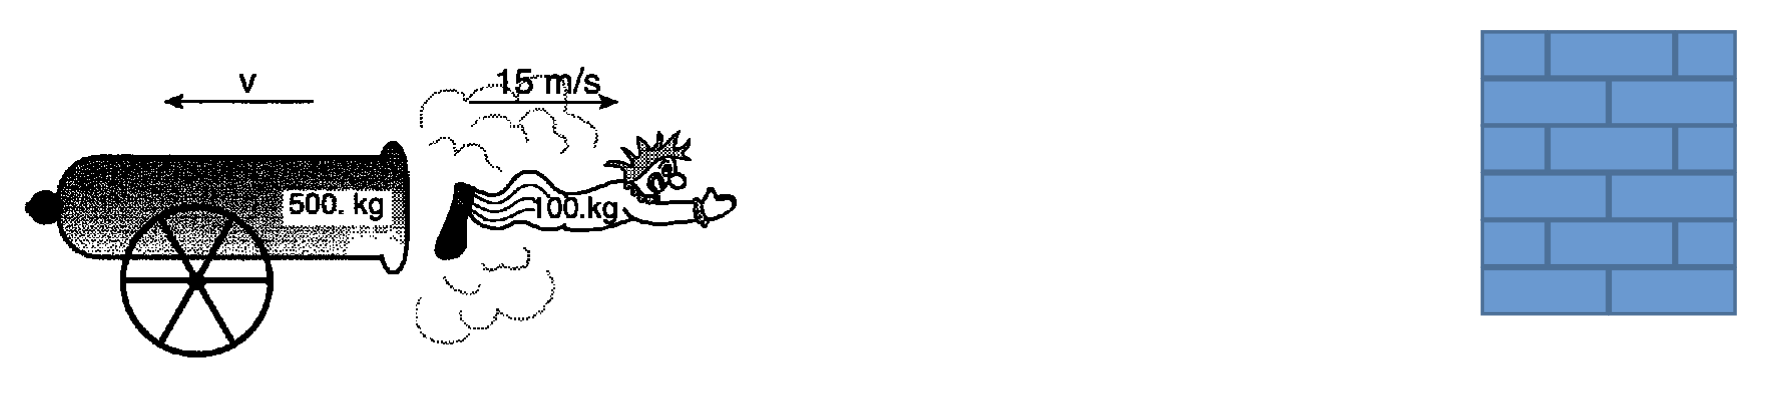
\includegraphics[width=4.7in]{images/clown.png}

\begin{questions}

\question
  What is the velocity of the cannon above? The cannon starts at rest and then fires out the clown at 15 m/s.  (If you can't read the picture, the cannon has a mass of 500~kg and the clown has a mass of 100~kg)
  \vspace{12em}

\question
  The clown (still traveling at 15 m/s) then hits a wall and comes to a stop in 0.85~seconds. What is the force acting on him?
\end{questions}
}

%%%%%%%%%%%%%%%%%%%%%%%%%%%%%%%%%%%%%%

\begin{document}
\pagestyle{empty}

\setlength{\columnsep}{0.8in}
\begin{multicols*}{2}

\noindent  
Name: \hfill Period: \hspace{5em}
\vspace{0.5em}
\hrule

\section*{\todayDate}
\subsection*{Warmup}

\content

\vfill
\hrule
\vspace{0.5em}
\hfill {\sc Physics I}

\columnbreak

\noindent  
Name: \hfill Period: \hspace{5em}
\vspace{0.5em}
\hrule

\section*{\todayDate}
\subsection*{Warmup}

\content

\vfill
\hrule
\vspace{0.5em}
\hfill {\sc Physics I}

\end{multicols*}

\end{document}